% Beamer
\documentclass{beamer}
\usetheme{Boadilla}

% Alignment
\usepackage{graphbox}

% Animation
\usepackage{animate}

% Font & encoding
\usepackage[utf8]{inputenc}
\usepackage[T1]{fontenc}
\usepackage{lmodern}
\usepackage{xcolor}
\hypersetup{unicode}
\hypersetup{breaklinks=true}

% Math
\usepackage{amsmath}
\usepackage{amsfonts}

% Custom commands
\renewcommand{\d}{\ensuremath{\mathrm d}}
\newcommand{\e}{\ensuremath{\mathrm e}}
\renewcommand{\i}{\ensuremath{\mathrm i}}
\newcommand{\R}{\ensuremath{\mathbb R}}
\renewcommand{\C}{\ensuremath{\mathbb C}}

\title[Magnetic Transport]{Magnetic Transport Along \\ Translationally Invariant Obstacles}
\subtitle{A Bachelor's Thesis Defense}
\author{Michal Grňo}
\date{\today}

\begin{document}

\begin{frame}
    \titlepage
\end{frame}

\begin{frame}
    \frametitle{Magnetic \color{gray} Transport Along \\ Translationally Invariant Obstacles}
    \pause
    A magnetic Hamiltonian
    \begin{equation*}
        H_0 = \big({ -\i\vec\nabla + \vec A }\big)^2 \: ,
    \end{equation*}
    \pause\vspace{-\baselineskip}
    \begin{equation*}
        \vec\nabla \times \vec A = \vec B_0 = \text{const.}
        \vspace{5pt}
    \end{equation*}
    \pause
    restricted to a 2D plane orthogonal to $\vec B_0$.
    \\\phantom{.}\\
    \pause
    This is the \textit{Landau Hamiltonian}.
\end{frame}

\begin{frame}
    \frametitle{{\color{gray}Magnetic Transport Along \\ Translationally Invariant} Obstacles}
    \begin{itemize}
        \pause
        \item potential obstacle: $H = H_0 + V(x,y)$
        \pause
        \item magnetic obstacle: $\vec B = \vec B_0 + \vec b(x,y)$\pause, $\; \vec b \parallel \vec B_0$
        \pause
        \item geometric obstacle:
        \begin{itemize}
            \item the system is not restricted to a plane, but to a \structure{thin layer}
            \pause
            \item the layer is smoothly \structure{bent}
            \pause
            \item Dirichlet boundary is assumed
        \end{itemize}
    \end{itemize}
\end{frame}

\begin{frame}
    \frametitle{{\color{gray}Magnetic Transport Along} \\ Translationally Invariant Obstacles}
    \begin{itemize}
        \item potential obstacle: $H = H_0 + \structure{V(x)}$
        \item magnetic obstacle: $\vec B = \vec B_0 + \structure{\vec b(x)}$, $\; \vec b \parallel \vec B_0$
        \item geometric obstacle:
        \begin{itemize}
            \item the system is not restricted to a plane, but to a thin layer
            \item the layer is smoothly bent and \structure{invariant under translation $y \mapsto y + c$}
            \item Dirichlet boundary is assumed
        \end{itemize}
    \end{itemize}
\end{frame}

\begin{frame}
    \frametitle{Magnetic Transport \color{gray} Along \\ Translationally Invariant Obstacles}
    \pause
    Classically:
    \begin{figure}
        \centering
        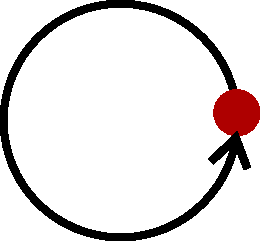
\includegraphics[scale=.5,align=c]{magnetic_localized.pdf}
        \hspace{2cm}
        \pause
        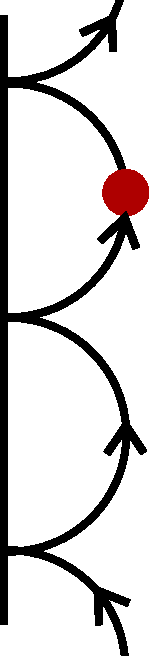
\includegraphics[scale=.5,align=c]{magnetic_skipping.pdf}
        \hspace{2cm}
        \pause
        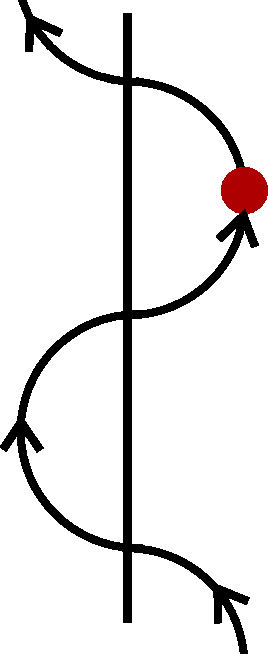
\includegraphics[scale=.5,align=c]{magnetic_snake.pdf}
     \end{figure}
\end{frame}

\begin{frame}
    \frametitle{Magnetic Transport \color{gray} Along \\ Translationally Invariant Obstacles}
    Quantum Mechanics: \\[15pt]
    \begin{itemize}
        \pause
        \item Spectrum of $H$ is pure point
        \begin{itemize}
            \pause
            \item[$\leftrightsquigarrow$] there is a basis consisting of stationary states
            \pause
            \item[$\leftrightsquigarrow$] time evolution is trivial \\[15pt]
        \end{itemize}
        \pause
        \item Spectrum of $H$ is continuous
        \begin{itemize}
            \pause
            \item[$\leftrightsquigarrow$] there are no stationary states
            \pause
            \item[$\leftrightsquigarrow$] \structure{\textbf{Magnetic Transport!}}
        \end{itemize}
    \end{itemize}
    \vspace*{2cm}
\end{frame}

\begin{frame}
    \frametitle{Magnetic Transport Along \\ Translationally Invariant Obstacles}
    The Hamiltonian is either of these:
    \\[15pt]
    \begin{enumerate}
        \item[(a)] $H = \big({ -\i\vec\nabla + \vec A }\big)^2 + V(x)$ on $L^2(\Omega \subset \R^2)$
        \item[(b)] $H = \big({ -\i\vec\nabla + \vec A(x)}\big)^2$ on $L^2(\Omega \subset \R^2)$
        \item[(c)] $H = \big({ -\i\vec\nabla + \vec A})$ on $L^2(\Omega)$, $\Omega$ being a thin layer in $\R^3$
        \\[15pt]
    \end{enumerate}
    And we are interested in its pure point / continuous spectrum.
\end{frame}

\begin{frame}
    \frametitle{The two parts}

    \begin{enumerate}
        \item Summary of known results
        \\[5pt]
        \begin{itemize}
            \item Steep potential wall (Macris et al., 1999) and (Fröhlich et al., 2000)
            \\[5pt]
            \item Half-plane with Dirichlet boundary (Fröhlich et al., 2000)
            \\[5pt]
            \item Bounded magnetic perturbation (Iwatsuka, 1983 and 1985)
            \\[5pt]
            \item Layer with one-sided fold, asymptotically flat layer, very thin layer (Exner et al., 2018)
            \\[15pt]
        \end{itemize}
        \pause
        \item Original work
        \\[5pt]
        \begin{itemize}
            \item Half-plane with Robin boundary
            \\[5pt]
            \item Dirac $\delta$-interaction on a line
        \end{itemize}
    \end{enumerate}
\end{frame}

\begin{frame}
    \frametitle{Frame Title}
    \centering
    \animategraphics[autoplay,loop,height=225pt]{1}{plots/robin}{1}{17}
\end{frame}

\begin{frame}
    \frametitle{Frame Title}
    \centering
    \animategraphics[autoplay,loop,height=225pt]{1}{plots/dirac}{1}{22}
\end{frame}


\end{document}
